\documentclass[12pt]{article}
\usepackage{booktabs}
\usepackage[authoryear,sort&compress]{natbib}
%\usepackage[numbers,sort&compress]{natbib}
\usepackage{amsmath,amsfonts,amssymb,amsbsy}
\usepackage{color}
\usepackage[colorlinks=true,citecolor=cyan,linkcolor=blue,urlcolor=magenta]{hyperref}
\usepackage{subfigure}
\usepackage{graphicx}
\usepackage{authblk}
\usepackage{parskip}
\usepackage{lineno}


\title{Introduction to \LaTeX}
%\author{Sara Mahallati\thanks{IBBME, University of Toronto, Canada; \texttt{t{tt{t{sara.mahallati@mail.utoronto.ca}}}

\author[1,2]{Sara Mahallati\thanks{sara.mahallati@mail.utoronto.ca}}
\author[3]{Dionne M. Aleman \thanks{This document is a modified version of the source file developed by Dr. Aleman}}
\affil[1]{Institute of Biomaterials and Biomedical Engineering, University of Toronto, Canada}
\affil[3]{Department of Mechanical and Industrial Engineering, University of Toronto}
\affil[2]{Krembil Research Institute, University Health Network, Toronto, Canada}


\date{June 21, 2018}


% THE ACTUAL DOCUMENT

\begin{document}

\maketitle
%\linenumbers

\begin{abstract}
This is a quick and dirty guide to doing most of the things most people will ever want to do with \LaTeX. This guide contains a number of examples of useful things (e.g., abstracts, arrows, tables, etc.) that may not be covered in the session today. Just look at the source \texttt{.tex} file to see how it was done (that is why there are a number of random bullets, symbols, sections, formatting styles, etc.\ throughout the guide). This document is certainly not the definitive \LaTeX\ manual; if there is something you want to do and it is not described here, look it up online. There are no limits to what can be done!  
\end{abstract}

\newpage

\tableofcontents

\newpage

\section*{Acknowledgement} %the * is added to make it an un-numbered section 
\addcontentsline{toc}{section}{Acknowledgement}
This source file is mostly adopted from Dr. Dionne Aleman's tutorial at MIE department a few years back and used with her permission. 

\section{What is \LaTeX ?} \label{sec:intro}

From \href{https://en.wikipedia.org/wiki/TeX}{wikipedia-tex}, \TeX\ (pronounced ``tek") is a typesetting system created by Donald Knuth. Together with the METAFONT language for font description and the Computer Modern typeface, it was designed with two main goals in mind: to allow anybody to produce high-quality books using a reasonable amount of effort, and to provide a system that would give the exact same results on all computers, now and in the future. Within the typesetting system, its name is formatted as \TeX.

% A message to help newbies avoid nit-picky pitfalls

\textbf{The key to being a proficient \LaTeX user is simple: Stop worrying about formatting, and just trust that \LaTeX\ will do it right for you.}



\subsection{Why use \LaTeX?}
\LaTeX\ can be difficult to learn, and most people are too hopelessly attached to Microsoft's products to try something new. If Word works pretty well, why change? Here's a breakdown of some of the more obvious pros and cons of \LaTeX.

\subsection{Pros and cons}

\paragraph{Pros} 
\begin{itemize}
	\item \LaTeX\ documents are beautiful. The typesetting, spacing and kerning are all perfect, and the font (Computer Modern) is infinitely scalable, so it looks sharp at any size.
	\item As shown in this document, you can create links to sections, tables, figures, citations, equations, bullets, URLs
	\item moreover, it's automatic! You will never again have to redo your section numbers because you reorganized a paper, or worse, redo your citations because you added in a new reference that throws off the numbering.
	\item You also won't have to redo your citations because the journal you are submitting your paper to wants a different citation format than what you used.
\end{itemize}  


For a strict comparison to Word, \TeX\ documents are just text, so they will never become bloated in file size (no matter how large your paper) or mysteriously crash and cause you to lose hours of work. \LaTeX\ won't make your pictures suddenly disappear while you tried to move the image one pixel upward. Your equations will look elegant and respectable, and not like they were written by a child. Further, equations are \textit{easy}---no more hunting for symbols and brackets in MathType. Tables are pure text, so you can automate table creation right from your data matrices in Matlab, C++, etc.


\paragraph{Cons} 
\begin{itemize}
	\item \LaTeX\ has a learning curve. Unlike Word, you can't really just start using it without spending some effort to learn what is going on. That's why we have this tutorial.
	\item Also unlike Word, \LaTeX\ won't let you (easily) do whatever you want in your document.\textbf{The driving vision behind \LaTeX\ is that \textit{it} will do your typesetting; you just do the typing.}. You are virtually not allowed to spend your time placing figures and tables exactly where you want them, because \LaTeX\ will generally put things where it thinks they go best. At first, this causes a lot of users headaches because they want to nitpick over positioning (and usually in an incorrect fashion). Eventually, you will realize that \LaTeX\ is in fact putting your floating objects in the best place they should be, and you will be happy not to have to worry about such things anymore.
	\item Possibly the biggest drawback to \LaTeX\ is that it does not have the reviewing toolbar that Word has, which allows you and collaborators to track changes made to a document. There are some ways to get around this if you are working with non-\LaTeX\ users (one way it to copy the paragraph you want to change into Word and then track the changes made), but nothing is very elegant.
\end{itemize}  

 
\section{How to install \LaTeX \ and editors}
In Section \ref{sec:intro}, we learned about \LaTeX. In Section \ref{sec:win}, we'll talk about how to get and install \LaTeX.

There are many different packages and editors available. TeXWorks is included in the distribution you download. The ones listed below are just ones I have used and liked, but there are certainly many other good ones. Most packages and editors are 100\% free. Just download and install the packages and editors, and you are ready to go.

\textit{PRO TIP: Install \LaTeX\ and any additional items first, then install your editor last. That way, your editor will probably auto-detect everything on its own.}




\subsection{Mac}

\begin{enumerate}
\item \LaTeX\ package
\begin{itemize}
\item MacTex: \url{http://www.tug.org/mactex/}
\end{itemize}
\item Editor
\begin{itemize}
\item TeXShop: \url{http://www.uoregon.edu/~koch/texshop/}
\end{itemize}
\end{enumerate}

\subsection{Windows OS} \label{sec:win}
\begin{itemize}
\item \LaTeX\ package
\begin{itemize}
\item MikTex: \url{http://miktex.org/}
\end{itemize}
\item Editor
\begin{itemize}
\item TeXstudio: \url{https://www.texstudio.org/}
\end{itemize}
\end{itemize}


\subsection{How to use the editors}
Once you have written your \LaTeX\ document\footnote{Look! A footnote! Did you notice that the footnote number in the text was a link to this footnote?}, you will ``typeset" (compile) your work. Your editor will automatically create a pdf document, along other auxiliary files. 

\section{How to write your \LaTeX\ document}
The rest of this document describes the basics of writing a paper in \LaTeX. This covers everything that 90\% of users will ever need, but only scratches the surface of what you can do. A famous comprehensive guide, ``The Not So Short Introduction to \LaTeX", details just about everything and can be found at
\begin{center}\url{http://www.ctan.org/tex-archive/info/lshort/english/lshort.pdf}\end{center}



\subsection{How to write mathematical equations}
\LaTeX\ makes writing mathematical equations ridiculously easy, and the results are picture-perfect. 

\subsubsection{Math inline with text}
To use math inline with text, type the equation inline with your text, and surround it by \$$\ldots$\$. The equation will automatically be formatted to best fit in the paragraph. For example, with $\sum_{i \in S} x_i \geq 1$, the subscript for the summation is placed to the side rather than underneath.


\subsubsection{Single equations}
You can write a single equation one of two ways:
\begin{enumerate}
\item \label{longhand} \verb!\begin{equation} ... \end{equation}!
\item \label{shorthand} \verb!$$ ... $$!
\end{enumerate}
where ``\ldots" represents the equation itself. Method \ref{shorthand} is essentially just shorthand for Method \ref{longhand} (look at the source document to see how these linked labels were made). For example, using Method \ref{longhand}:
\begin{equation} 
\label{eqn:f} F(\Theta) = \mu + \epsilon(\theta)
\end{equation}
yields the same result as Method \ref{shorthand}:
$$ F(\Theta) = \mu + \epsilon(\theta) $$
Note that Method \ref{shorthand} does not number the equation. Equation \ref{eqn:f} is numbered.

\paragraph{Pro tip} When writing equations, \textbf{do not skip lines} in your source code. A skipped line in the source document is interpreted as a new paragraph, and if you skip a line before your equation, there will be too much vertical spacing before the equation in the \texttt{pdf}. Skipping lines after the equation is fine if you intend whatever content comes next to be a new paragraph.

\subsubsection{Numbering equations}
Equations are automatically numbered, but if you don't want to number an equation, either use the shorthand method or place an asterisk (\texttt{*}) after \texttt{equation} in both the begin and end statements.

\begin{equation*} 
F(\Theta) = \mu + \epsilon(\theta)
\end{equation*}


\subsubsection{Matrices/arrays}
Matrices are just arrays displayed with brackets around them. For example:

\begin{equation}
\mathbf{R} = \left[ 
\begin{array}{cc}
a & b  \\
c & d  \\
e & f  \\
\end{array} 
\right], 
\end{equation}

\begin{equation}
\mathbf{R} = \left( 
\begin{array}{ccc}
a_1 & \cdots & z_1 \\
\vdots & \ddots & \vdots \\
a_n & \cdots & z_n
\end{array} 
\right). 
\end{equation}

Dots are created using \verb!\cdots! (center dots), \verb!\vdots! (vertical dots) and \verb!\ddots! (diagonal dots). Ellipses-style dots are created by \verb!\ldots! (lower dots).

Using \verb!\left(! and \verb!\right)! will create parentheses that expand to the appropriate size to fit the content inside them. The ( and ) can be replaced with any other bracketing-type symbol with the same effect. A \verb!\left! must ALWAYS be accompanied by a  \verb!\right!. To only use the left or right bracket/brace/etc., use a ``." instead of the omitted bracket/brace/etc. symbol.
\begin{equation*}
y_i = \left\{ \begin{array}{ll}
1 & \mbox{if facility is built at location } i \\
0 & \mbox{otherwise}
\end{array} \right.
\end{equation*}


\subsubsection{Greek letters}
If you can spell the names of Greek letters, you can easily use them in \LaTeX. 

\paragraph{Lowercase letters}
Lowercase Greek letters are simply $\backslash$name, where ``name" is the name of the letter in all lowercase. For example:
\begin{eqnarray*}
\backslash\mbox{gamma} &\rightarrow& \gamma \\
\backslash\mbox{delta} &\rightarrow& \delta \\
\backslash\mbox{pi} &\leftarrow& \pi \\
\backslash\mbox{phi} &\leftarrow& \phi \\
\end{eqnarray*}

\paragraph{Uppercase letters}
Uppercase Greek letters are simply $\backslash$Name, where ``Name" is the name of the letter in with the first letter capitalized. For example:
\begin{eqnarray*}
\backslash\mbox{Gamma} &\Rightarrow& \Gamma \\
\backslash\mbox{Delta} &\Rightarrow& \Delta \\
\backslash\mbox{Pi} &\Leftarrow& \Pi \\
\backslash\mbox{Phi} &\Leftarrow& \Phi \\
\end{eqnarray*}


\subsection{Figures}
Figures are fairly easy, and new \LaTeX\ distributions no longer mandate eps or pdf format (though eps and pdf are generally better for scaling). You can save your figures as eps files. make sure that any font in your figure (e.g., legends) is legible. This usually means that the fonts will have to be seemingly unreasonably large.

\begin{figure}[tbp]
	\centering 
	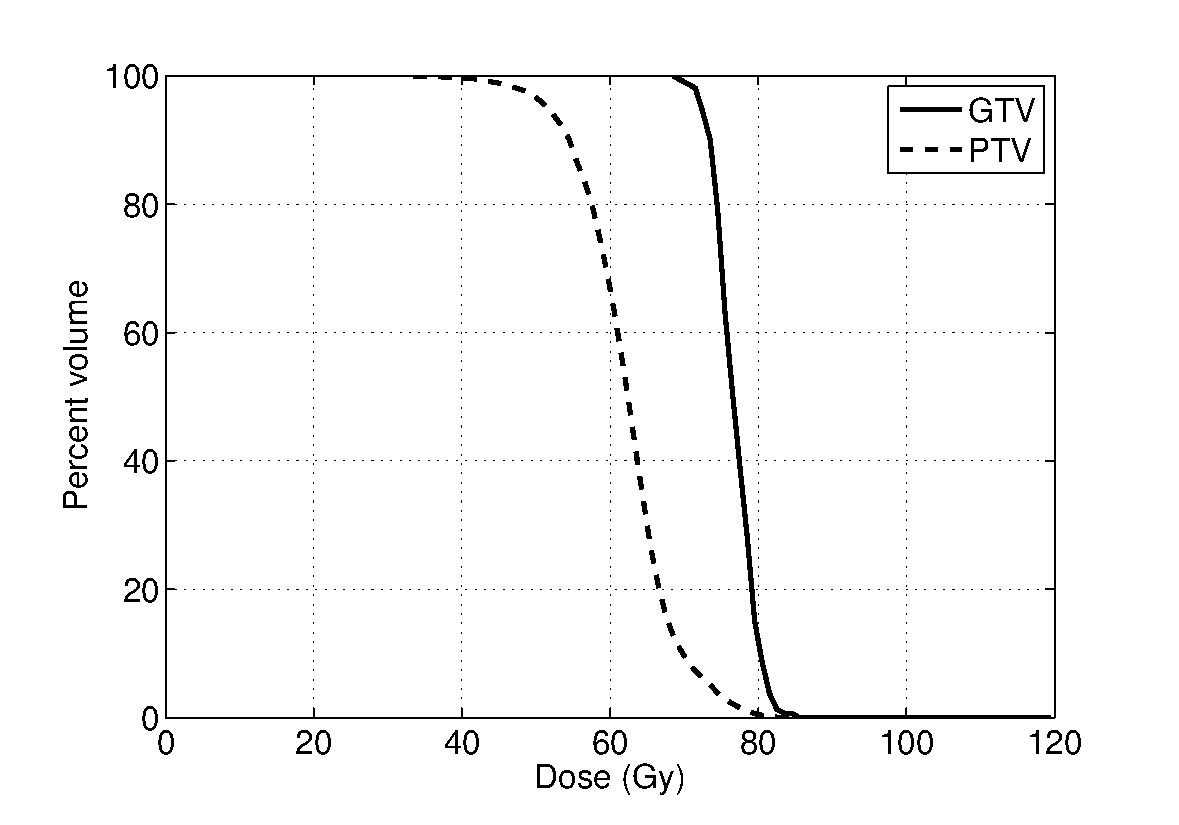
\includegraphics[width=0.75\textwidth]{graph}
	\caption{Graphical results} 
	\label{fig:DVHs}
\end{figure}

We can also easily create subfigures using the \texttt{subfigure} package. We can then refer to them as Figure \ref{fig:cluster-pre} and Figure \ref{fig:cluster-post}, or refer to the whole figure set as Figure \ref{fig:cluster}.

\begin{figure}[tbp]
	\begin{center}
		\subfigure[Contour plot of iteration $k$]{
			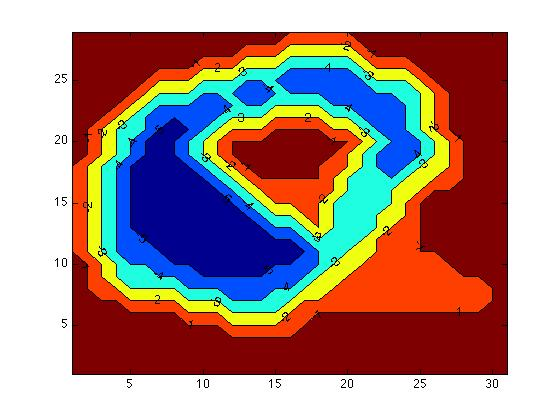
\includegraphics[scale=0.4]{contour1.jpg}
			\label{fig:cluster-pre}
		}
		\subfigure[Contour plot of iteration $k+1$]{
			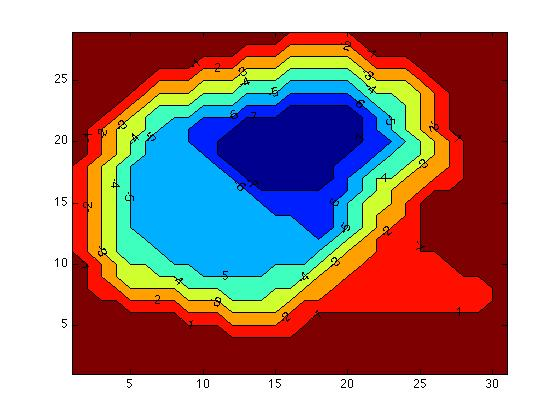
\includegraphics[scale=0.4]{contour2.jpg}
			\label{fig:cluster-post}
		}
	\end{center}
	\caption{Contour plots of the target at two subsequent iterations of the skeletonization algorithm.}
	\label{fig:cluster}
\end{figure}

Look at the code to generate Figures \ref{fig:DVHs} and \ref{fig:cluster} in the \texttt{tex} file. Note that the width can be specified as a percentage of the total text width (\verb![width=0.75\textwidth]!) or as a scale of the original figure size (\verb![scale=0.4]!). 

\subsection{Citations}
Citations in \LaTeX \ are done through another package called BibTeX, which should come pre-installed with your \LaTeX\ package. Simply write the information for all the publications you want to cite in a text file with extension \texttt{.bib}, and then include that file (without extension) and a particular citation style as a bibliography at the end of your document:

\begin{verbatim}
\bibliographystyle{plain}
\bibliography{bibfile_latex_howto}
\end{verbatim}

To reference a single publication \citep{Mahallati2018}, simply write the citation's key inside a \verb!\cite{}! command:
\begin{verbatim}
\cite{Mahallati2018}
\end{verbatim}
For multiple citations like \cite{Buzsaki2012, Peyrache2012, Mahallati2018a}:
\begin{verbatim}
\cite{Buzsaki2012, Peyrache2012, Anastassiou2015}
\end{verbatim}
Unless told otherwise, BibTeX will order your bibliography by last name of first author and then by year. Section \ref{sec:citeorder} shows how to automatically sort and compress your citations.

For fancier citations (e.g., ``name, year" format), use the \verb!natbib! package and change the bibliography style from \verb!plain! to something else. Rather than make your own style, it easier to find a journal whose style you like, and then download their citation style (which is usually publicly available).

\subsubsection{Sorting and compressing citations} \label{sec:citeorder}
It is generally considered very bad form to have your citations appear in non-alphabetical or non-numerical order. But, it can be tedious to re-arrange your citations or insert new citations if you have a string of several reference. Compressing citations (e.g., [1--4,7] instead of [1,2,3,4,7]) can also be time-consuming. Fortunately, the \texttt{natbib} package will automatically take care of that.

Just include the \texttt{natbib} package in your header with options to either sort or sort and compress:
\begin{verbatim}
\usepackage[sort]{natbib}
\usepackage[sort&compress]{natbib}
\end{verbatim}
Note that compressing will only change the citation appearance if you are using numbered citations.

\subsubsection{Compiling citations}
To get your references to show up, you will have to:
\begin{enumerate}
	\item Typeset your document with \LaTeX: tells the editor which publications from your \texttt{.bib} file you want to cite;
	\item Typeset your document with BibTeX: formats the citations according to your bibliography style;
	\item Typeset your document with \LaTeX\ twice more: figures out what numbering each citation should have (usually based on last name of first author) and puts it all in your document.
\end{enumerate}

Some editors actually compiles both \LaTeX\ and BibTeX simultaneously, so you effectively have to compile the document 3-4 times to get the in-text citations updated.

The same principle of multiple compilations applies to generating the table of contents and figure/table numbers, as well as to section, equation, table and figure referencing.

\subsubsection{Making your citations into links}
Your references to bibliography items and to other sections can be turned into actually hyperlinks in the document by using the \verb!hyperref! package. Nothing different needs to be done in terms of citing references or referring to sections, tables or figures; just include the package in the document header.

See the source code of this document for an example of how to set colors.

%%%%%%%%%%%%%%%%%%%%%%%%%%%%%%%%%%%%%
\subsection{Tables}
Tables are a little bit of work in \LaTeX. Table \ref{tbl:vals} uses a plain layout. Alternatively, you can use the table styles defined in the \verb!booktabs! package for a more polished look as in Table \ref{tbl:fancyvals}.

Although the creation of tables is not as intuitive as in, say, Microsoft Excel, the pure text format certainly has its advantages. For example, if you have a matrix of values in Matlab (or any other programming environment/language) that you want to put in a table in your document, you don't have to copy those values over by hand. Just write a quick function that will read in the matrix and print out the ampersands (\verb!&!) and endlines (\verb!\\!) appropriately. Regardless of how large your table is, you just have to call one function and your table is ready for you to paste into your \verb!.tex! file!


\begin{table}[tbp] % t = top, b = bottom, p = own page, h = here (not recommended)
\centering
\begin{tabular}{|c|rr|rr|}  % l = left, c = center, r = right
\hline
 & \multicolumn{2}{c|}{\textbf{Obj. fn. value}} & \multicolumn{2}{c|}{\textit{Run time (hrs)}} \\
\hline
case &	Avg. & St. Dev. & Avg. & St. Dev. \\
\hline\hline
1 &	565.24 &	8.82 &	5.35 &	5.07 \\
2 &	570.51 &	12.83 &	7.49 &	3.78 \\
3 &	893.45 &	20.60 &	7.05 &	2.21 \\
4 &	710.92 &	7.72 &	6.54 &	3.39 \\
5 &	512.22 &	20.04 &	6.96 & 	3.33 \\
6 &	799.95 &	34.07 &	3.48 &	3.40 \\
\hline
\end{tabular}
\caption{Minimum objective function values and time computation time.}
\label{tbl:vals}
\end{table}


\begin{table}[tbp]
\centering
\begin{tabular}{c @{ \hspace{1cm} } cc @{\hspace{1cm}} cc @{\hspace{0.5cm}}}
\toprule
 & \multicolumn{2}{l}{\textit{Obj. fn. value}} & \multicolumn{2}{c}{\textit{Run time (hrs)}} \\
case & Average & St. Dev. & Average & St. Dev. \\ 
\midrule
1 &	565.24 &	8.82 &	5.35 &	5.07 \\
2 &	570.51 &	12.83 &	7.49 &	3.78 \\
3 &	893.45 &	20.60 &	7.05 &	2.21 \\
4 &	710.92 &	7.72 &	6.54 &	3.39 \\
5 &	512.22 &	20.04 &	6.96 & 	3.33 \\
6 &	799.95 &	34.07 &	3.48 &	3.40 \\
\bottomrule
\end{tabular}
\caption{A nicer layout of the table. Note the extra spacing placed between columns.}
\label{tbl:fancyvals}
\end{table}


\section{\LaTeX\ instead of PowerPoint}
\LaTeX\ can be used a presentation medium as well through a package called Beamer:
\begin{center} \url{http://bitbucket.org/rivanvx/beamer/wiki/Home} \end{center}
One of the great benefits of Beamer, aside from preventing the use of animations, is the dynamic presentation outline that allows your audience to see exactly where in the presentation you are at any given moment.

More information on how to use Beamer can be found at the link above, but it basically boils down to putting 
\begin{verbatim}
\frame{
\frametitle{Your frame title}
...
}
\end{verbatim}
around your content.




% THE REFERENCES
\bibliographystyle{abbrvnat}
%\bibliographystyle{plain}
%\bibliography{bibfile_latex_howto}
\bibliography{MyLibrary}

\newpage

% THE APPENDIX
\appendix

\section{Tables of data} \label{app:tabledata}
Look, an appendix! You can reference an appendix just like anything else. See the code in Appendix \ref{app:tabledata} for examples.

\newpage

\section{Figures upon figures} \label{app:figs}
Another appendix! This one is automatically named Appendix \ref{app:figs}.



\end{document}
